
% Copyright (c) 2015 - 2020 Mario Mlačak, mmlacak@gmail.com
% Licensed and published as Public Domain work.

% One chapter =========================================================
\chapter*{One}
\addcontentsline{toc}{chapter}{One}

\begin{flushright}
\parbox{0.8\textwidth}{
\emph{God is not external to anyone, but is present with all things, though
they are ignorant that he is so. \\
\hspace*{\fill}{\textperiodcentered \textperiodcentered \textperiodcentered \hspace*{0.2em} Plotinus} } }
\end{flushright}

\noindent
One is chess variant which is played on 26 x 26 board, with white and
darker violet fields, and with light purple and fuchsia pieces. Star
colors are reversed colors of ordinary pieces, i.e. fuchsia and light
purple. In algebraic notation, columns are enumerated from 'a' to 'z',
and rows are enumerated from '1' to '26'. A new piece is introduced,
Starchild.

\clearpage % ..........................................................
% Starchild ***********************************************************

\section*{Starchild}
\addcontentsline{toc}{section}{Starchild}

\noindent
\begin{wrapfigure}[11]{l}{0.4\textwidth}
\centering
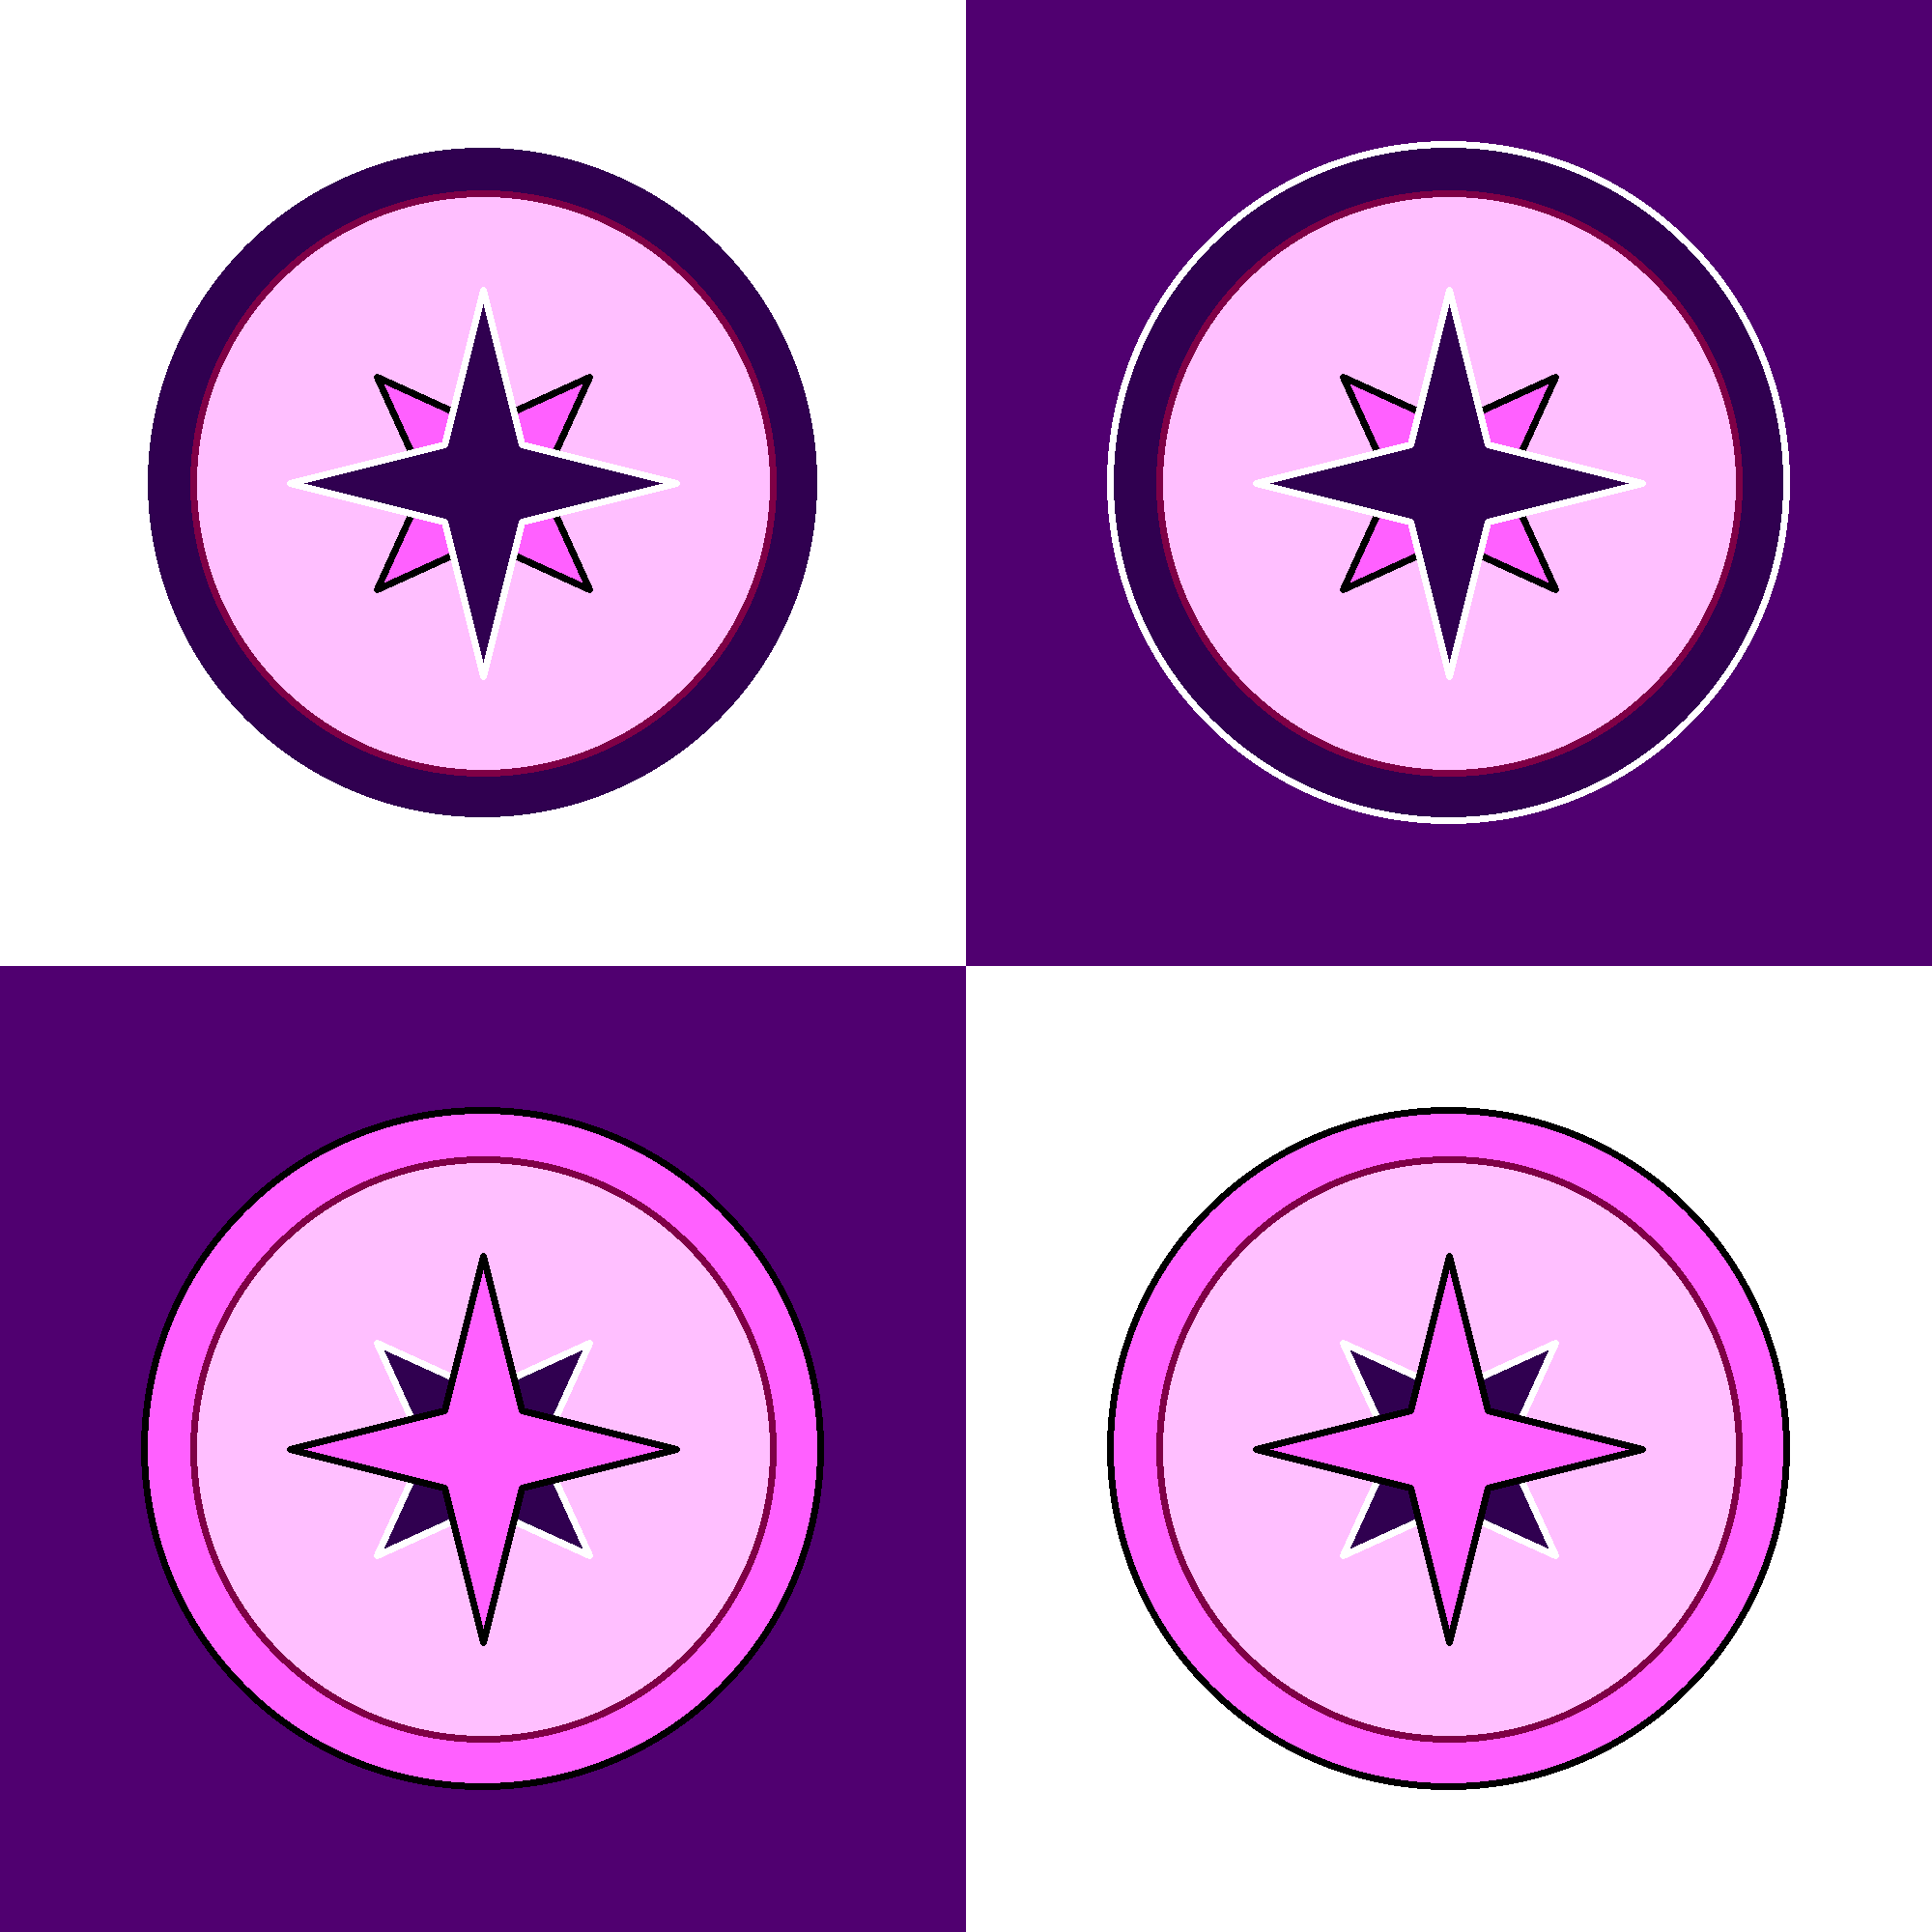
\includegraphics[width=0.4\textwidth, keepaspectratio=true]{pieces/16_starchild.png}
\caption{Starchild}
\label{fig:16_starchild}
\end{wrapfigure}
Starchild is supporting piece, it cannot capture any piece, cannot check or checkmate
opponent's King.

Starchild cannot be converted, but can be activated. If activated, it does not spend
momentum while moving. Starchild can activate any own piece, except King, and can
activate opponent's Starchilds. Starchild can also activate and move Stars, but not
Monoliths.

Starchild can take any piece, except Kings, Stars and Monoliths, for a non-interactive,
viewing-only trance-journey.

% \vspace*{0.15\textheight}
\noindent
\begin{wrapfigure}[10]{l}{0.4\textwidth}
\centering
\includegraphics[width=0.4\textwidth, keepaspectratio=true]{pieces/star/22_one.png}
\caption{Star}
\label{fig:star/22_one}
\end{wrapfigure}
Starchild can't teleport. Starchild moves from starting to empty destination field in
an instant, without ever stepping on any intermediate fields and without interacting
with any pieces on them.

Starchild can ressurect any captured piece.

In algebraic notation, symbol for Starchild is 'I'.

Star colors in this variant are presented above, on the left.

\clearpage % ..........................................................
% Movement ------------------------------------------------------------

\subsection*{Movement}
\addcontentsline{toc}{subsection}{Movement}

\vspace*{-1.1\baselineskip}
\noindent
\begin{figure}[!h]
% \begin{figure}[!t]
\includegraphics[width=1.0\textwidth, keepaspectratio=true]{examples/22_o/scn_o_01_starchild_movement.png}
\caption{Starchild movement}
\label{fig:scn_o_01_starchild_movement}
% \centering
\end{figure}

Starchild can move to any empty field in opposite color to the one it's located on.
Starchild is not hampered by any piece between starting and destination field.

Here, light Starchild in the middle is positioned at dark field, and so can access
any empty light field on chessboard, in a single move.

\clearpage % ..........................................................

\subsection*{Neighboring-fields}
\addcontentsline{toc}{subsection}{Neighboring-fields}

\vspace*{-0.9\baselineskip}
\noindent
\begin{wrapfigure}[5]{l}{0.4\textwidth}
\centering
\includegraphics[width=0.192307692\textwidth, keepaspectratio=true]{examples/22_o/scn_o_02_neighboring_fields.png}
\caption{Neighboring-fields}
\label{fig:scn_o_02_neighboring_fields}
\end{wrapfigure}
Neighboring-fields are all fields immediately surrounding a piece horizontally, vertically
and diagonally. They are the same as step-fields of a King.

\vspace*{1.1\baselineskip}
\subsection*{Activating piece}
\addcontentsline{toc}{subsection}{Activating piece}

\vspace*{-0.9\baselineskip}
\noindent
\begin{wrapfigure}[7]{l}{0.4\textwidth}
\centering
\includegraphics[width=0.192307692\textwidth, keepaspectratio=true]{examples/22_o/scn_o_03_starchild_activating_fields.png}
\caption{Activating piece}
\label{fig:scn_o_03_starchild_activating_fields}
\end{wrapfigure}
Fields at which Starchild can activate a piece are neighboring-fields.

Note, Starchild can move only to non-empty activation fields, and only if it contains
own piece, except King, or opponent's Starchids.

Here, Starchild’s activation fields are enumerated. Opponent's Bishop and own King can't
be activated, so only own Pegasus can be, with 1 momentum.

\vspace*{-1.1\baselineskip}
\subsection*{Moving a Star}
\addcontentsline{toc}{subsection}{Moving a Star}

\vspace*{-0.9\baselineskip}
\noindent
\begin{wrapfigure}[5]{l}{0.4\textwidth}
\centering
\includegraphics[width=0.192307692\textwidth, keepaspectratio=true]{examples/22_o/scn_o_04_starchild_moving_star_init.png}
\caption{Moving into a Star}
\label{fig:scn_o_04_starchild_moving_star_init}
\end{wrapfigure}
Starchild's activation fields are enumerated. Starchild can move a Star by activating it,
the same way as any other piece, i.e. by capturing field at which Star is located.

\clearpage % ..........................................................

% \vspace*{2.1\baselineskip}
\noindent
\begin{wrapfigure}[4]{l}{0.4\textwidth}
\centering
\includegraphics[width=0.192307692\textwidth, keepaspectratio=true]{examples/22_o/scn_o_05_starchild_moving_star_end.png}
\caption{Moving a Star}
\label{fig:scn_o_05_starchild_moving_star_end}
\end{wrapfigure}
Once activated, Star can move to any empty neighboring-field, which all are enumerated in
example on the left.

\vspace*{2.1\baselineskip}
\subsection*{Not moving a Monolith}
\addcontentsline{toc}{subsection}{Not moving a Monolith}

\vspace*{-0.9\baselineskip}
\noindent
\begin{wrapfigure}[5]{l}{0.4\textwidth}
\centering
\includegraphics[width=0.192307692\textwidth, keepaspectratio=true]{examples/22_o/scn_o_06_starchild_not_moving_monolith_init.png}
\caption{Moving into a Monolith}
\label{fig:scn_o_06_starchild_not_moving_monolith_init}
\end{wrapfigure}
Starchild’s activation fields are enumerated. Starchild can try to capture field at which
Monolith is located, as if trying to activate and move it.

\vspace*{2.1\baselineskip}
% \vspace*{3.9\baselineskip}
\noindent
\begin{wrapfigure}[4]{l}{0.4\textwidth}
\centering
\includegraphics[width=0.192307692\textwidth, keepaspectratio=true]{examples/22_o/scn_o_07_starchild_not_moving_monolith_end.png}
\caption{Moving out of a Monolith}
\label{fig:scn_o_07_starchild_not_moving_monolith_end}
\end{wrapfigure}
Instead of moving a Monolith, Starchild then emerges on any empty portal-field around Monolith
it tried to move.

\clearpage % ..........................................................

% \vspace*{3.7\baselineskip}
\subsection*{Trance-journey}
\addcontentsline{toc}{subsection}{Trance-journey}

\vspace*{-0.9\baselineskip}
\noindent
\begin{wrapfigure}[12]{l}{0.4\textwidth}
\centering
\includegraphics[width=0.346153846\textwidth, keepaspectratio=true]{examples/22_o/scn_o_08_trance_journey_init.png}
\caption{Starting a trance-journey}
\label{fig:scn_o_08_trance_journey_init}
\end{wrapfigure}
Trance-journey is initiated by either Shaman (A steps) or Starchild (B), by activating a
Starchild. Activated Starchild then activates a piece, entranced piece then leaves onto
trance-journey. Any piece, own or opponent's, can be entranced, except Kings, Stars and
Monoliths. Entraced piece must have the same color as initiating Shaman or Starchild,
color of entrancing Starchild do not need to match. Trance-journey is optional, last
piece could just move.

Initiating Shaman or Starchild can themselves be activated by some other piece(s), not necessarily in the same color.

\clearpage % ..........................................................



\clearpage % ..........................................................

[*] Syzygy (+?) ... --\textgreater ressurection [*]

[*] TODO :: Star moved \textgreater\textgreater Wave cannot pass through ... teleportation is mandatory (not optional!) [*]

[*] moved Star ---\textgreater Wave \textgreater\textgreater if no board field beyond other Star \textgreater\textgreater sacrified [*]
see \hyperref[fig:scn_d_11_wave_teleported_off_board]{see "Wave teleported off-board"}

% ------------------------------------------------------------ Movement
% *********************************************************** Starchild
\clearpage % ..........................................................

\section*{Promotion}
\addcontentsline{toc}{section}{Promotion}

Promotion is non enforced, delayed variety, i.e. it's the same as in
\hyperref[sec:Age of Aquarius/Promotion]{previous chess variant}, Age of Aquarius.

Additionaly, promotion in this variant is monogamous.
Only one Queen in the same color can be present on chessboard at any given time.

\clearpage % ..........................................................

\section*{Rush, en passant}
\addcontentsline{toc}{section}{Rush, en passant}

\vspace*{-1.2\baselineskip}
\noindent
\begin{figure}[!h]
% \begin{figure}[!t]

\includegraphics[width=1.0\textwidth, keepaspectratio=true]{en_passants/22_one_en_passant.png}
\caption{En passant}
\label{fig:22_one_en_passant}
% \centering
\end{figure}

Rush and en passant are identical to those in \hyperref[fig:14_hemera_s_dawn_en_passant]{Hemera's Dawn variant}.
Own Pawns can be rushed for up to 11 fields in this variant.

\clearpage % ..........................................................

\section*{Castling}
\addcontentsline{toc}{section}{Castling}

Castling is the same as in Classical Chess, only difference is that King can move between 2 and 10 fields across.
All other constraints from Classical Chess still applies.

\noindent
\begin{figure}[!h]
% \begin{figure}[!t]
\includegraphics[width=1.0\textwidth, keepaspectratio=true]{castlings/22_o/one_castling.png}
\caption{Castling}
\label{fig:one_castling}
% \centering
\end{figure}

In example above, all valid King's castling moves are numbered.

\noindent
\begin{figure}[!h]
% \begin{figure}[!t]
\includegraphics[width=1.0\textwidth, keepaspectratio=true]{castlings/22_o/one_castling_right_04.png}
\caption{Castling short right}
\label{fig:one_castling_right_04}
% \centering
\end{figure}

In this example King was castling short to the right. Initial King's position is marked with "K".
After castling is finished, right Rook ends up at field immediately left to the King.

\clearpage % ..........................................................

\section*{Initial setup}
\addcontentsline{toc}{section}{Initial setup}

Compared to initial setup of Discovery, Starchild is inserted between Unicorn and Shaman
symmetrically, on both sides of chessboard. This can be seen in the image below:

\noindent
% \begin{figure}[t]
\begin{figure}[h]
\includegraphics[width=1.0\textwidth, keepaspectratio=true]{boards/22_one.png}
\caption{One board}
\label{fig:22_one}
% \centering
\end{figure}

\clearpage % ..........................................................
% ========================================================= One chapter
